% !TeX program = xelatex
\documentclass[a4paper,10pt]{article}

% ============================================================================
% សន្លឹកកិច្ចការសិស្សបំពេញចន្លោះ ស-ខ្មៅ និងប្លង់ក្ដារខៀន/ចម្លើយគ្រូ (គ្មាន LCD / គ្មានកន្ត្រៃ)
% មេរៀនទី៣ (២.៧)៖ ការទិញបណ្ដាក់ — ត្រូវគ្នា ១០០% នឹង LS_Plan_INS327.tex
% ============================================================================
\usepackage[a4paper, left=1.0cm, right=1.0cm, top=0.75cm, bottom=1.00cm, footskip=0.52cm]{geometry}
\usepackage{amsmath}
\usepackage{unicode-math}
\usepackage{fontspec}
\usepackage{array, colortbl}
\usepackage[table]{xcolor}
\usepackage{enumitem}
\usepackage{pifont}
\usepackage{fancyhdr}
\usepackage{lastpage}
\usepackage{tikz}
\usepackage[most]{tcolorbox}
\usetikzlibrary{calc, arrows.meta, decorations.pathreplacing, positioning, babel}

\makeatletter
\let\@expl@@@mark@update@singlecol@structures@@\relax
\makeatother

\providecommand{\NGSFindFonts}{%
  \IfFileExists{C:/Windows/Fonts/cambria.ttc}{%
    \def\NGSSysPath{C:/Windows/Fonts/}%
    \def\NGSUserPath{C:/Users/KIT/AppData/Local/Microsoft/Windows/Fonts/}%
  }{%
    \IfFileExists{./fonts/KhmerOSsiemreap.ttf}{\def\NGSSysPath{./fonts/}\def\NGSUserPath{./fonts/}}{%
    \IfFileExists{../fonts/KhmerOSsiemreap.ttf}{\def\NGSSysPath{../fonts/}\def\NGSUserPath{./fonts/}}{%
    \IfFileExists{../../fonts/KhmerOSsiemreap.ttf}{\def\NGSSysPath{../../fonts/}\def\NGSUserPath{../../fonts/}}{%
    \IfFileExists{../../../fonts/KhmerOSsiemreap.ttf}{\def\NGSSysPath{../../../fonts/}\def\NGSUserPath{../../../fonts/}}{%
    \IfFileExists{../../../../fonts/KhmerOSsiemreap.ttf}{\def\NGSSysPath{../../../../fonts/}\def\NGSUserPath{../../../../fonts/}}{%
    \IfFileExists{../../../../../fonts/KhmerOSsiemreap.ttf}{\def\NGSSysPath{../../../../../fonts/}\def\NGSUserPath{../../../../../fonts/}}{%
    \IfFileExists{../../../../../../fonts/KhmerOSsiemreap.ttf}{\def\NGSSysPath{../../../../../../fonts/}\def\NGSUserPath{../../../../../../fonts/}}{%
      \def\NGSSysPath{../../../../../../../fonts/}\def\NGSUserPath{../../../../../../../fonts/}%
    }}}}}}}%
  }%
}
\NGSFindFonts

\setmathfont[Path={\NGSSysPath}, FontIndex=1, Scale=1.02]{cambria.ttc}
\defaultfontfeatures{Ligatures=TeX}

\setmainfont[
  Path={\NGSUserPath}, Extension=.ttf, Script=Khmer,
  BoldFont={KhmerOSsiemreap}, BoldFeatures={FakeBold=1.8},
  ItalicFont={KhmerOSsiemreap}, ItalicFeatures={FakeSlant=0.25},
  BoldItalicFont={KhmerOSsiemreap}, BoldItalicFeatures={FakeBold=1.8, FakeSlant=0.25}
]{KhmerOSsiemreap}

\newfontfamily\muol[Path={\NGSUserPath}, Extension=.ttf, Script=Khmer]{KhmerOSmuollight}
\newfontfamily\TimesEn[Path={\NGSSysPath}, Extension=.ttf, BoldFont={timesbd}, ItalicFont={timesi}, BoldItalicFont={timesbi}]{times}
\newfontfamily\CalibriFont[Path={\NGSSysPath}, Extension=.ttf]{calibri}

\XeTeXlinebreaklocale "km"
\XeTeXlinebreakskip = 0pt plus 1pt minus 0.1pt

\definecolor{panelgray}{gray}{0.94}
\definecolor{headgray}{gray}{0.85}
\definecolor{midgray}{gray}{0.76}

\pagestyle{fancy}
\fancyhf{}
\renewcommand{\headrulewidth}{0pt}
\fancyfoot[L]{\fontsize{7.4pt}{9.5pt}\selectfont អនុវិទ្យាល័យព្រះក្រសាំង \en{|} គ្រូ៖ ហុក ប៊ុនថែន \en{|} មេរៀនទី៣ (២\en{.}៧) ការទិញបណ្ដាក់ \en{|} ថ្ងៃព្រហស្បតិ៍ ទី២៦ ខែវិច្ឆិកា ឆ្នាំ២០២៦}
\fancyfoot[R]{\fontsize{7.8pt}{10pt}\selectfont ទំព័រ \en{\thepage\ / \pageref{LastPage}}}

\setlength{\parindent}{0pt}
\setlength{\parskip}{0pt}
\setlength{\tabcolsep}{4pt}

\newcommand{\en}[1]{{\TimesEn #1}}
\newcommand{\enbf}[1]{{\TimesEn\bfseries #1}}
\newcommand{\unit}[1]{\,\text{\en{#1}}}
\newcommand{\riel}{\,\text{៛}}
\newcommand{\usd}{\,\text{\en{\$}}}
\newcommand{\cnum}[1]{\mbox{\fontsize{10pt}{12pt}\selectfont\ding{\numexpr181+#1\relax}}}
\newcommand{\chkbox}{\tikz[baseline=-0.15ex]\draw[black, line width=0.85pt, fill=white] (0,0) rectangle (0.24cm,0.24cm);}
\newcommand{\ansbox}[1][1.75cm]{\,\tikz[baseline=-0.65ex]\draw[black, line width=0.65pt, fill=white] (0,0) rectangle (#1, 0.42cm);\,}
\newcommand{\dotline}[1][2.2cm]{\makebox[#1]{\dotfill}}

\newcommand{\pagebanner}[2]{%
  \begin{tcolorbox}[
    enhanced, sharp corners, colback=headgray, colframe=black,
    boxrule=1.05pt, boxsep=1pt, top=2.5pt, bottom=2.5pt, left=6pt, right=6pt,
    after skip=3.5pt
  ]
    {\muol\fontsize{9.0pt}{13.2pt}\selectfont #1}\hfill{\fontsize{8.0pt}{11.2pt}\selectfont\textbf{#2}}
  \end{tcolorbox}%
}

\newcommand{\secstrip}[2]{%
  \vspace{3pt}%
  \begin{tcolorbox}[
    enhanced, sharp corners, colback=panelgray, colframe=black,
    boxrule=0.8pt, boxsep=0.8pt, top=2pt, bottom=2pt, left=5pt, right=5pt,
    after skip=3pt
  ]
    {\muol\fontsize{8.5pt}{12.2pt}\selectfont #1}\hfill{\fontsize{7.8pt}{10.8pt}\selectfont\textit{#2}}
  \end{tcolorbox}%
}

\newcolumntype{L}[1]{>{\raggedright\arraybackslash}p{#1}}
\newcolumntype{C}[1]{>{\centering\arraybackslash}p{#1}}

\begin{document}
\fontsize{9.5pt}{14.5pt}\selectfont

% ============================================================================
% ទំព័រទី ១៖ សន្លឹកកិច្ចការសិស្ស (ផ្នែកមុខ៖ E1 -> E2 -> E3)
% ============================================================================
\pagebanner{សន្លឹកកិច្ចការសិស្ស \enbf{(}២\enbf{.}៧ ការទិញបណ្ដាក់\enbf{)} \enbf{--} ផ្នែកមុខ}{ថ្នាក់ទី៨ \en{|} សៀវភៅគោល ទំ.៣៨--៣៩}

\begin{tcolorbox}[
  enhanced, sharp corners, colback=white, colframe=black,
  boxrule=0.8pt, boxsep=1.5pt, top=3.5pt, bottom=3.5pt, left=5pt, right=5pt,
  after skip=4pt
]
  \fontsize{9.0pt}{13.0pt}\selectfont
  \textbf{ឈ្មោះសិស្ស៖} \dotline[4.3cm] \quad
  \textbf{សមាជិកក្រុម៖} \dotline[4.3cm] \quad
  \textbf{ថ្នាក់ទី៖} ៨\dotline[0.9cm] \quad
  \textbf{ក្រុមទី៖} \dotline[1.0cm]
\end{tcolorbox}

% --- E1 Engage ---
\secstrip{ផ្នែកទី ១ \enbf{(E1 - Engage)} ៖ បេសកកម្មស្លាកតម្លៃម៉ូតូបណ្ដាក់ ($4\,000\,000\riel$, កក់ $1\,000\,000\riel$)}{រយៈពេល ៣ នាទី (គូស \ding{51} ក្នុង \chkbox)}

\begin{tcolorbox}[
  enhanced, sharp corners, colback=white, colframe=black,
  boxrule=0.8pt, boxsep=2pt, top=3.5pt, bottom=3.5pt, left=6pt, right=6pt
]
  ហាងលក់ម៉ូតូមួយដាក់លក់ម៉ូតូថ្លៃមិនបណ្ដាក់ $4\,000\,000\riel$ ឬទិញបណ្ដាក់ដោយកក់មុន $1\,000\,000\riel$ ហើយគិតការប្រាក់ $10\%$/ឆ្នាំ រយៈពេល $2$ ឆ្នាំ ($24$ ខែ) ៖\\[2pt]
  $\bullet$ \textbf{តើហាងត្រូវគិតការប្រាក់តាមមតិណា?} \quad
  \chkbox\ \textbf{មតិទី ១៖} គិតលើថ្លៃដើមទាំង $4\,000\,000\riel$ \qquad
  \chkbox\ \textbf{មតិទី ២៖} គិតតែលើប្រាក់នៅជំពាក់ $3\,000\,000\riel$\\[2pt]
  $\bullet$ \textbf{ហេតុផលខ្លី៖} ហេតុអ្វីប្រាក់កក់ $1\,000\,000\riel$ មិនត្រូវគិតការប្រាក់ទៀត? \dotline[6.4cm] ។
\end{tcolorbox}

\vfill

% --- E2 Explore ---
\secstrip{ផ្នែកទី ២ \enbf{(E2 - Explore)} ៖ ដ្យាក្រាមលំហូរ ៤ ដំណាក់នៃការទិញបណ្ដាក់ (ទំ.៣៨--៣៩)}{រយៈពេល ១១ នាទី}

\textbf{សកម្មភាព ១ (\en{E2-A} — ៦ នាទី)៖ ឧទាហរណ៍ទិញកុំព្យូទ័រថ្លៃមិនបណ្ដាក់ $P_{\text{ដើម}} = 9\,000\,000\riel$, កក់ $D = 2\,000\,000\riel$, អត្រា $R = 14\%$/ឆ្នាំ, $2$ ឆ្នាំ ($24$ ខែ)}

\begin{tcolorbox}[
  enhanced, sharp corners, colback=white, colframe=black,
  boxrule=0.8pt, boxsep=2pt, top=3.5pt, bottom=3.5pt, left=6pt, right=6pt
]
  $\bullet$ \textbf{ដំណាក់ \cnum{1} — ប្រាក់នៅជំពាក់ ($B$)៖} $B = P_{\text{ដើម}} - D = 9\,000\,000 - 2\,000\,000 =$ \ansbox[2.4cm] $\riel$\\[3pt]
  $\bullet$ \textbf{ដំណាក់ \cnum{2} — ការប្រាក់លើប្រាក់នៅជំពាក់ ($2$ ឆ្នាំ)៖} $I = \dfrac{B \times 14 \times 2}{100} =$ \dotline[2.4cm] $\riel$\\[2pt]
  \hspace*{0.4cm}$\implies$ ប្រាក់នៅជំពាក់បូកការប្រាក់សរុប៖ $S = B + I =$ \dotline[2.2cm] $+$ \dotline[2.2cm] $=$ \ansbox[2.4cm] $\riel$\\[3pt]
  $\bullet$ \textbf{ដំណាក់ \cnum{3} — ប្រាក់សងរំលស់ប្រចាំខែ ($m = 24$ ខែ)៖} $M = \dfrac{S}{24} =$ \dotline[2.4cm] $\div 24 \approx$ \ansbox[2.5cm] $\riel$/ខែ
\end{tcolorbox}

\vspace{3pt}
\textbf{សកម្មភាព ២ (\en{E2-B} — ៥ នាទី)៖ អន្ទាក់ភ្លេចដកប្រាក់កក់ និងថ្លៃទិញបណ្ដាក់សរុប (ដំណាក់ \cnum{4})}

\begin{tcolorbox}[
  enhanced, sharp corners, colback=white, colframe=black,
  boxrule=0.8pt, boxsep=2pt, top=3.5pt, bottom=3.5pt, left=6pt, right=6pt
]
  $\bullet$ \textbf{ពិនិត្យអន្ទាក់៖} បើសិស្សម្នាក់ភ្លេចដកប្រាក់កក់ ហើយគិតការប្រាក់ $14\%$ រយៈពេល $2$ ឆ្នាំ លើ $9\,000\,000\riel$ ទាំងមូល នោះការប្រាក់ឡើងដល់ \dotline[2.3cm] $\riel$ (លើសការពិតចំនួន \dotline[2.1cm] $\riel$!) ។\\[3pt]
  $\bullet$ \textbf{ដំណាក់ \cnum{4} — ថ្លៃទិញបណ្ដាក់សរុប៖} $P_{\text{បណ្ដាក់}} = D + S = 2\,000\,000 +$ \dotline[2.3cm] $=$ \ansbox[2.4cm] $\riel$\\[2pt]
  $\bullet$ \textbf{កម្មសិទ្ធិ (ទំ.៣៨)៖} អ្នកទិញក្លាយជាម្ចាស់ទំនិញពេញសិទ្ធិ នៅពេលបង់ប្រាក់សងរំលស់ \dotline[2.8cm] ។
\end{tcolorbox}

\vfill

% --- E3 Explain ---
\secstrip{ផ្នែកទី ៣ \enbf{(E3 - Explain)} ៖ រូបមន្តការទិញបណ្ដាក់ និងធនាគារហេតុផល \enbf{B\&W}}{រយៈពេល ៦ នាទី}

\begin{tcolorbox}[
  enhanced, sharp corners, colback=white, colframe=black,
  boxrule=0.85pt, boxsep=2pt, top=3.5pt, bottom=3.5pt, left=6pt, right=6pt
]
  ១) \textbf{ប្រាក់នៅជំពាក់៖} $B = P_{\text{ដើម}} - \dotline[1.0cm]$ \qquad
  ២) \textbf{ប្រាក់សងរំលស់សរុប៖} $S = B + \dotline[1.0cm]$ \ ($I = \frac{B\times R\times T}{100}$)\\[3pt]
  ៣) \textbf{សងរំលស់ប្រចាំខែ ($m$ ខែ)៖} $M = \dfrac{S}{\dotline[0.9cm]}$ \qquad
  ៤) \textbf{ថ្លៃបណ្ដាក់សរុប៖} $P_{\text{បណ្ដាក់}} = D + S = D + m\times \dotline[0.9cm]$\\[4pt]
  \tikz\draw[black, dashed, line width=0.5pt] (0,0) -- (18.4cm,0);\\[3pt]
  \fontsize{8.8pt}{12.8pt}\selectfont
  \textbf{ធនាគារហេតុផល (\en{Warrant Bank})៖} \quad
  \cnum{1} \textbf{ដកប្រាក់កក់ជាមុន៖} $B = P_{\text{ដើម}} - D$ \quad
  \cnum{2} \textbf{ការប្រាក់លើ $B$៖} $I = \frac{B\cdot R\cdot T}{100} \implies S = B + I$\\
  \cnum{3} \textbf{ចែកចំនួនខែ $m$៖} $M = \frac{S}{m}$ \quad
  \cnum{4} \textbf{ថ្លៃបណ្ដាក់សរុប និង $\%$ បន្ថែម៖} $P_{\text{បណ្ដាក់}} = D + S$; \ $\% = \frac{P_{\text{បណ្ដាក់}} - P_{\text{ដើម}}}{P_{\text{ដើម}}}\times 100\%$
\end{tcolorbox}

% ============================================================================
% ទំព័រទី ២៖ សន្លឹកកិច្ចការសិស្ស (ផ្នែកខាងខ្នង៖ E4 -> E5 -> កិច្ចការផ្ទះ)
% ============================================================================
\clearpage
\pagebanner{សន្លឹកកិច្ចការសិស្ស \enbf{(}២\enbf{.}៧ ការទិញបណ្ដាក់\enbf{)} \enbf{--} ផ្នែកខាងខ្នង}{ថ្នាក់ទី៨ \en{|} សៀវភៅគោល ទំ.៣៩--៤០, ៤២}

% --- E4 Elaborate ---
\secstrip{ផ្នែកទី ៤ \enbf{(E4 - Elaborate)} ៖ លំហាត់គំរូទី ១ — ម៉ាស៊ីនបោកខោអាវ (ទំ.៣៩)}{រយៈពេល ១០ នាទី}

\begin{tcolorbox}[
  enhanced, sharp corners, colback=white, colframe=black,
  boxrule=0.8pt, boxsep=2pt, top=3.5pt, bottom=3.5pt, left=6pt, right=6pt
]
  \textbf{លំហាត់គំរូទី ១ (ទំ.៣៩)៖} ម៉ាស៊ីនបោកខោអាវថ្លៃមិនបណ្ដាក់ $P_{\text{ដើម}} = 1\,350\,000\riel$ ។ បើទិញបណ្ដាក់ ត្រូវកក់មុន $15\%$ និងបង់ការប្រាក់លើប្រាក់នៅសល់តាមអត្រា $10\frac{2}{3}\% = \frac{32}{3}\%$ ក្នុង ១ ឆ្នាំ សម្រាប់រយៈពេល $2$ ឆ្នាំ ($24$ ខែ) ៖\\[3pt]
  $\bullet$ \textbf{ដំណាក់ \cnum{1}៖} ប្រាក់កក់ $D = \frac{15}{100}\times 1\,350\,000 =$ \dotline[2.0cm] $\riel \implies$ ប្រាក់នៅជំពាក់ $B =$ \dotline[2.2cm] $\riel$\\[3pt]
  $\bullet$ \textbf{ដំណាក់ \cnum{2}៖} ការប្រាក់ $I = B \times \frac{32}{3} \times \frac{1}{100} \times 2 =$ \dotline[2.0cm] $\riel \implies S = B + I =$ \dotline[2.2cm] $\riel$\\[3pt]
  $\bullet$ \textbf{ក) សងរំលស់ប្រចាំខែ (\cnum{3})៖} $M = S \div 24 =$ \dotline[2.0cm] $\riel \approx$ \ansbox[2.0cm] $\riel$ \quad
  \textbf{ខ) ថ្លៃបណ្ដាក់សរុប (\cnum{4})៖} $P_{\text{បណ្ដាក់}} =$ \ansbox[2.2cm] $\riel$\\[3pt]
  $\bullet$ \textbf{គ) ប្រាក់សន្សំបានបើទិញមិនបណ្ដាក់៖} \dotline[2.0cm] $\riel \implies$ គិតជាភាគរយនៃថ្លៃដើម $= \dfrac{\dotline[1.6cm]}{1\,350\,000}\times 100\% =$ \ansbox[2.1cm] $\%$\\[2pt]
  \fontsize{8.7pt}{12.5pt}\selectfont
  \textbf{ឆ្លុះបញ្ចាំង (\en{EIA Looking-Back})៖} បើប្រធានប្រាប់ $D, M$ និងចំនួនខែ $m$ ស្រាប់ គេរកថ្លៃបណ្ដាក់សរុបតាម $P_{\text{បណ្ដាក់}} = D +$ \dotline[1.6cm] ។
\end{tcolorbox}

\vfill

% --- E5 Evaluate ---
\secstrip{ផ្នែកទី ៥ \enbf{(E5 - Evaluate)} ៖ តារាងប្រតិបត្តិ (ទំ.៤០) សំណួរវិនិច្ឆ័យ \enbf{A--D} និងសំបុត្រចេញ}{រយៈពេល ១០ នាទី}

\begin{tcolorbox}[
  enhanced, sharp corners, colback=white, colframe=black,
  boxrule=0.8pt, boxsep=2pt, top=3pt, bottom=3pt, left=5pt, right=5pt
]
  \textbf{១) ប្រតិបត្តិ (ទំ.៤០)៖} រកចំនួនប្រាក់បន្ថែម និងសម្ដែងជាភាគរយនៃតម្លៃទិញមិនបណ្ដាក់ ៖\\[3pt]
  \centering
  {\fontsize{8.7pt}{12.5pt}\selectfont\renewcommand{\arraystretch}{1.24}
  \begin{tabular}{|C{0.7cm}|C{2.4cm}|C{2.0cm}|C{2.4cm}|C{1.4cm}|L{3.5cm}|L{4.2cm}|}
    \hline
    \cellcolor{headgray}\textbf{ល.រ} &
    \cellcolor{headgray}\textbf{ថ្លៃមិនបណ្ដាក់} &
    \cellcolor{headgray}\textbf{ប្រាក់កក់} &
    \cellcolor{headgray}\textbf{រំលស់ប្រចាំខែ} &
    \cellcolor{headgray}\textbf{ចំនួនខែ} &
    \cellcolor{headgray}\textbf{ថ្លៃបណ្ដាក់សរុប ($P_{\text{បណ្ដាក់}}$)} &
    \cellcolor{headgray}\textbf{ប្រាក់បន្ថែម និងភាគរយ ($\%$)} \\
    \hline
    ក & $1\,080\,000\riel$ & $150\,000\riel$ & $120\,000\riel$ & $10$ & \dotline[2.8cm] $\riel$ & \dotline[1.8cm] $\riel$ (\dotline[1.1cm] $\%$) \\
    \hline
    ខ & $2\,700\,000\riel$ & $450\,000\riel$ & $225\,000\riel$ & $12$ & \dotline[2.8cm] $\riel$ & \dotline[1.8cm] $\riel$ (\dotline[1.1cm] $\%$) \\
    \hline
  \end{tabular}}\\[3pt]
  \raggedright\fontsize{8.8pt}{12.6pt}\selectfont
  \textbf{២) បិទបេសកកម្ម \en{E1} (ម៉ូតូ $4\,000\,000\riel$, កក់ $1\,000\,000\riel$, $10\%$/ឆ្នាំ, $2$ ឆ្នាំ)៖} $B = 3\,000\,000\riel \implies I =$ \dotline[1.8cm] $\riel \implies M =$ \dotline[1.8cm] $\riel$/ខែ ។
\end{tcolorbox}

\vspace{3.5pt}

\begin{tcolorbox}[
  enhanced, sharp corners, colback=white, colframe=black,
  boxrule=0.8pt, boxsep=2pt, top=3.5pt, bottom=3.5pt, left=6pt, right=6pt
]
  \textbf{៣) សំណួរវិនិច្ឆ័យ \en{A--D} (ទិញកង់ថ្លៃដើម $600\,000\riel$ កក់ $100\,000\riel$ រំលស់ $62\,000\riel$/ខែ ចំនួន $10$ ខែ — លើកម្រាមដៃ ១--៤)៖}\\[2.5pt]
  \textbf{\en{A.}} សរុប $620\,000\riel$, បន្ថែម $20\,000\riel$ \quad
  \textbf{\en{B.}} សរុប $720\,000\riel$, បន្ថែម $120\,000\riel$ \quad
  \textbf{\en{C.}} សរុប $520\,000\riel$ \quad
  \textbf{\en{D.}} បន្ថែម $620\,000\riel$\\[3.5pt]
  \tikz\draw[black, dashed, line width=0.5pt] (0,0) -- (18.4cm,0);\\[3pt]
  \textbf{៤) សំបុត្រចេញ ៦០ វិនាទី៖} ទូរស័ព្ទថ្លៃដើម $800\,000\riel$ កក់ $200\,000\riel$ ការប្រាក់ $10\%$/ឆ្នាំ រយៈពេល $1$ ឆ្នាំ ($12$ ខែ)៖
  $B =$ \dotline[1.6cm] $\riel$, $I =$ \dotline[1.5cm] $\riel$, $M =$ \dotline[1.6cm] $\riel$/ខែ, $P_{\text{បណ្ដាក់}} =$ \dotline[1.8cm] $\riel$ ។
\end{tcolorbox}

\vfill

% --- Homework ---
\begin{tcolorbox}[
  enhanced, sharp corners, colback=panelgray, colframe=black,
  boxrule=0.95pt, boxsep=2pt, top=3.5pt, bottom=3.5pt, left=6pt, right=6pt
]
  {\muol\fontsize{9.0pt}{13.0pt}\selectfont កិច្ចការផ្ទះ \enbf{(}សៀវភៅគោល ទំ.៤២ លេខ ១៩ ក និង ខ\enbf{)}}\\[2.5pt]
  \fontsize{8.8pt}{13.0pt}\selectfont
  $\bullet$ \textbf{\#19 (ទំ.៤២)៖} ពូគាទិញម៉ាស៊ីនត្រជាក់មួយគ្រឿងដោយបណ្ដាក់ ។ ម៉ាស៊ីនត្រជាក់នោះថ្លៃ $2\,700\,000\riel$ គាត់ត្រូវកក់ប្រាក់ $20\%$ ហើយប្រាក់ដែលនៅជំពាក់ត្រូវសងក្នុងរយៈពេល $48$ ខែ ជាមួយអត្រាការប្រាក់ប្រចាំឆ្នាំ $10\%$ ។ \textbf{(ក)} រកប្រាក់ដែលត្រូវសងប្រចាំខែ; \quad \textbf{(ខ)} តើពូគាអាចសន្សំប្រាក់បានប៉ុន្មាន បើគាត់ទិញដោយមិនជំពាក់? \textbf{អានមុន៖} មេរៀនទី៤ រង្វាស់រង្វាល់ — ១. ផ្ទៃក្រឡានិងមាឌ (ទំ.៤៣--៤៤) ។
\end{tcolorbox}

% ============================================================================
% ទំព័រទី ៣៖ ទំព័រគ្រូបង្រៀន (គំរូប្លង់ក្ដារខៀន ៣ ផ្នែក + ចម្លើយផ្ទៀងផ្ទាត់រហ័ស)
% ============================================================================
\clearpage
\pagebanner{ទំព័រគ្រូបង្រៀន ៖ ប្លង់ក្ដារខៀន \enbf{(}គ្មាន \enbf{LCD)} និងចម្លើយផ្ទៀងផ្ទាត់រហ័ស}{២.៧ ការទិញបណ្ដាក់ (\en{INS327})}

\secstrip{១. គំរូប្លង់បែងចែកក្ដារខៀន ៣ ផ្នែក សម្រាប់ថ្នាក់រៀនគ្មាន \enbf{LCD}}{សម្រាប់គ្រូប្រើដីស/ហ្វឺត}

\begin{center}
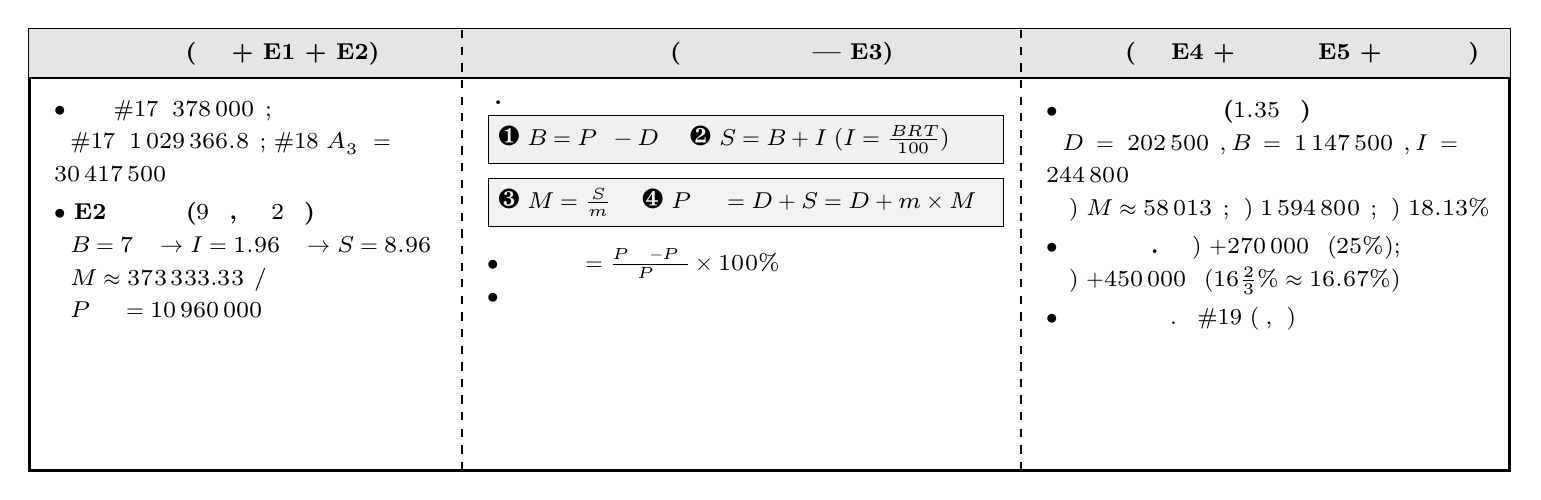
\begin{tikzpicture}[x=1cm, y=1cm, every node/.style={font=\fontsize{8.3pt}{11.8pt}\selectfont, text=black}]
  \draw[black, line width=1.1pt] (0,0) rectangle (18.8,5.60);
  \fill[gray!20] (0,4.98) rectangle (18.8,5.60);
  \draw[black, line width=0.7pt] (0,4.98) -- (18.8,4.98);
  \draw[black, dashed, line width=0.7pt] (5.5,0) -- (5.5,5.60);
  \draw[black, dashed, line width=0.7pt] (12.6,0) -- (12.6,5.60);

  \node at (2.75,5.29) {\textbf{ផ្នែកឆ្វេង (កំណែ + \en{E1} + \en{E2})}};
  \node at (9.05,5.29) {\textbf{ផ្នែកកណ្ដាល (ខ្លឹមសារគោលរក្សាទុក — \en{E3})}};
  \node at (15.70,5.29) {\textbf{ផ្នែកស្ដាំ (គំរូ \en{E4} + ប្រតិបត្តិ \en{E5} + កិច្ចការផ្ទះ)}};

  % Left
  \node[anchor=north west, text width=5.1cm] at (0.20,4.82) {%
    $\bullet$ \textbf{កំណែ៖} \#17ក $378\,000\riel$;\\
    \hspace*{0.2cm}\#17ខ $1\,029\,366.8\riel$; \#18 $A_3=30\,417\,500\riel$\\[2pt]
    $\bullet$ \textbf{\en{E2} កុំព្យូទ័រ ($9$លាន, កក់ $2$លាន)៖}\\
    \hspace*{0.2cm}$B=7$លាន $\to I=1.96$លាន $\to S=8.96$លាន\\
    \hspace*{0.2cm}$M \approx 373\,333.33\riel$/ខែ\\
    \hspace*{0.2cm}$P_{\text{បណ្ដាក់}} = 10\,960\,000\riel$
  };

  % Center
  \node[anchor=north west, text width=6.7cm] at (5.70,4.82) {%
    {\muol\fontsize{8.5pt}{12pt}\selectfont ២\enbf{.}៧ ការទិញបណ្ដាក់}\\[3pt]
    \tikz\node[draw=black, fill=gray!12, inner sep=3.5pt, text width=6.3cm]{%
      \cnum{1} $B = P_{\text{ដើម}} - D$ \quad \cnum{2} $S = B + I$ ($I = \frac{BRT}{100}$)
    };\\[4pt]
    \tikz\node[draw=black, fill=gray!10, inner sep=3.5pt, text width=6.3cm]{%
      \cnum{3} $M = \frac{S}{m}$ \quad \cnum{4} $P_{\text{បណ្ដាក់}} = D + S = D + m\times M$
    };\\[4pt]
    $\bullet$ ភាគរយបន្ថែម $= \frac{P_{\text{បណ្ដាក់}} - P_{\text{ដើម}}}{P_{\text{ដើម}}}\times 100\%$\\
    $\bullet$ សងរំលស់អស់ ទើបក្លាយជាម្ចាស់កម្មសិទ្ធិ
  };

  % Right
  \node[anchor=north west, text width=5.8cm] at (12.80,4.82) {%
    $\bullet$ \textbf{គំរូទី១ ម៉ាស៊ីនបោកខោអាវ ($1.35$លាន)៖}\\
    \hspace*{0.2cm}$D=202\,500\riel, B=1\,147\,500\riel, I=244\,800\riel$\\
    \hspace*{0.2cm}ក) $M \approx 58\,013\riel$; ខ) $1\,594\,800\riel$; គ) $18.13\%$\\[2pt]
    $\bullet$ \textbf{ប្រតិបត្តិ ទំ.៤០៖} ក) $+270\,000\riel$ ($25\%$);\\
    \hspace*{0.2cm}ខ) $+450\,000\riel$ ($16\frac{2}{3}\% \approx 16.67\%$)\\[2pt]
    $\bullet$ \textbf{កិច្ចការផ្ទះ៖} ទំ.៤២ \#19 (ក, ខ)
  };
\end{tikzpicture}
\end{center}

\vspace{4pt}
\secstrip{២. ចម្លើយផ្ទៀងផ្ទាត់រហ័សសម្រាប់សន្លឹកកិច្ចការសិស្ស \enbf{(}ទំព័រ ១ និង ទំព័រ ២\enbf{)}}{\en{Answer Key}}

\begin{tcolorbox}[
  enhanced, sharp corners, colback=white, colframe=black,
  boxrule=0.8pt, boxsep=2pt, top=4pt, bottom=4pt, left=6pt, right=6pt
]
  \fontsize{9.0pt}{13.6pt}\selectfont
  $\bullet$ \textbf{ផ្នែក \en{E1}៖} \textbf{មតិទី ២} ត្រឹមត្រូវ (គិតការប្រាក់តែលើប្រាក់នៅជំពាក់ $3\,000\,000\riel$ ព្រោះ $1\,000\,000\riel$ បានបង់រួចហើយ) ។\\[2pt]
  $\bullet$ \textbf{ផ្នែក \en{E2}៖} \textbf{សកម្មភាព ១៖} $B = 7\,000\,000\riel, I = 1\,960\,000\riel, S = 8\,960\,000\riel, M \approx 373\,333.33\riel$/ខែ ។ \textbf{សកម្មភាព ២៖} បើគិតលើ $9\,000\,000\riel$ បាន $2\,520\,000\riel$ (លើស $560\,000\riel$); $P_{\text{បណ្ដាក់}} = 10\,960\,000\riel$; បង់សងរំលស់\textbf{គ្រប់ចំនួនទាំងអស់} ។\\[2pt]
  $\bullet$ \textbf{ផ្នែក \en{E4}៖} $D = 202\,500\riel, B = 1\,147\,500\riel, I = 244\,800\riel, S = 1\,392\,300\riel$; ក) $58\,012.5 \approx 58\,013\riel$; ខ) $1\,594\,800\riel$; គ) $244\,800\riel \implies 18\frac{2}{15}\% \approx 18.13\%$ ។\\[2pt]
  $\bullet$ \textbf{ផ្នែក \en{E5}៖} \textbf{១) ប្រតិបត្តិ៖} (ក) $P_{\text{បណ្ដាក់}} = 1\,350\,000\riel$, បន្ថែម $270\,000\riel$ ($25\%$); (ខ) $P_{\text{បណ្ដាក់}} = 3\,150\,000\riel$, បន្ថែម $450\,000\riel$ ($16\frac{2}{3}\% \approx 16.67\%$) ។ \textbf{២) បិទ \en{E1}៖} $I = 600\,000\riel \implies M = 150\,000\riel$/ខែ ។ \textbf{៣) វិនិច្ឆ័យ \en{A--D}៖} \textbf{ជម្រើស \en{B}} ($720\,000\riel$, បន្ថែម $120\,000\riel$) ។ \textbf{៤) សំបុត្រចេញ៖} $B = 600\,000\riel, I = 60\,000\riel, M = 55\,000\riel$/ខែ, $P_{\text{បណ្ដាក់}} = 860\,000\riel$ ។
\end{tcolorbox}

\vspace{4pt}
\secstrip{៣. ចម្លើយលម្អិតនៃកិច្ចការផ្ទះ \enbf{(}សម្រាប់ផ្ទៀងនៅដើមម៉ោងបន្ទាប់ មេរៀនទី៤\enbf{)}}{សៀវភៅគោល ទំ.៤២}

\begin{tcolorbox}[
  enhanced, sharp corners, colback=white, colframe=black,
  boxrule=0.8pt, boxsep=2pt, top=4pt, bottom=4pt, left=6pt, right=6pt
]
  \fontsize{8.9pt}{13.4pt}\selectfont
  $\bullet$ \textbf{\#19 (ទំ.៤២ — ពូគាទិញម៉ាស៊ីនត្រជាក់ថ្លៃ $2\,700\,000\riel$, កក់ $20\%$, រំលស់ $48$ ខែ, អត្រា $10\%$/ឆ្នាំ)៖}\\[2pt]
  \hspace*{0.3cm}-- ប្រាក់កក់ $D = \frac{20}{100}\times 2\,700\,000 = 540\,000\riel \implies$ ប្រាក់នៅជំពាក់ $B = 2\,700\,000 - 540\,000 = 2\,160\,000\riel$ ។\\[2pt]
  \hspace*{0.3cm}-- រយៈពេល $48\text{ ខែ} = \frac{48}{12} = 4\text{ ឆ្នាំ} \implies$ ការប្រាក់ $I = \frac{2\,160\,000\times 10\times 4}{100} = 864\,000\riel \implies S = 2\,160\,000 + 864\,000 = 3\,024\,000\riel$ ។\\[2pt]
  \hspace*{0.3cm}-- \textbf{(ក) ប្រាក់ត្រូវសងប្រចាំខែ៖} $M = \frac{3\,024\,000}{48} = \mathbf{63\,000\riel}$/ខែ; \quad \textbf{(ខ) ប្រាក់សន្សំបើទិញមិនជំពាក់៖} $P_{\text{បណ្ដាក់}} = 540\,000 + 3\,024\,000 = 3\,564\,000\riel \implies$ សន្សំបាន $3\,564\,000 - 2\,700\,000 = \mathbf{864\,000\riel}$ ។
\end{tcolorbox}

\end{document}
